\newpage
\chapter{Flight Test}
\label{chap:flight_test}

\section{Flight Objectives and Planning}
%write for each subsystem

For the \ac{EPS}, the main test objectives were to: 
%
\begin{itemize}
\item Test if suitable power could be supplied to the motors for steering and forward propulsion
\item Confirm plausibility of providing all power from solar cells, i.e. estimate required amount of propulsion power
\item In-flight functional test of EPS telemetry and telecommand 
\end{itemize}
%
%
\section{Flight Results}
\label{sec:flight_results}
%write for each subsystem
%
%
\begin{figure}[H]
\centering
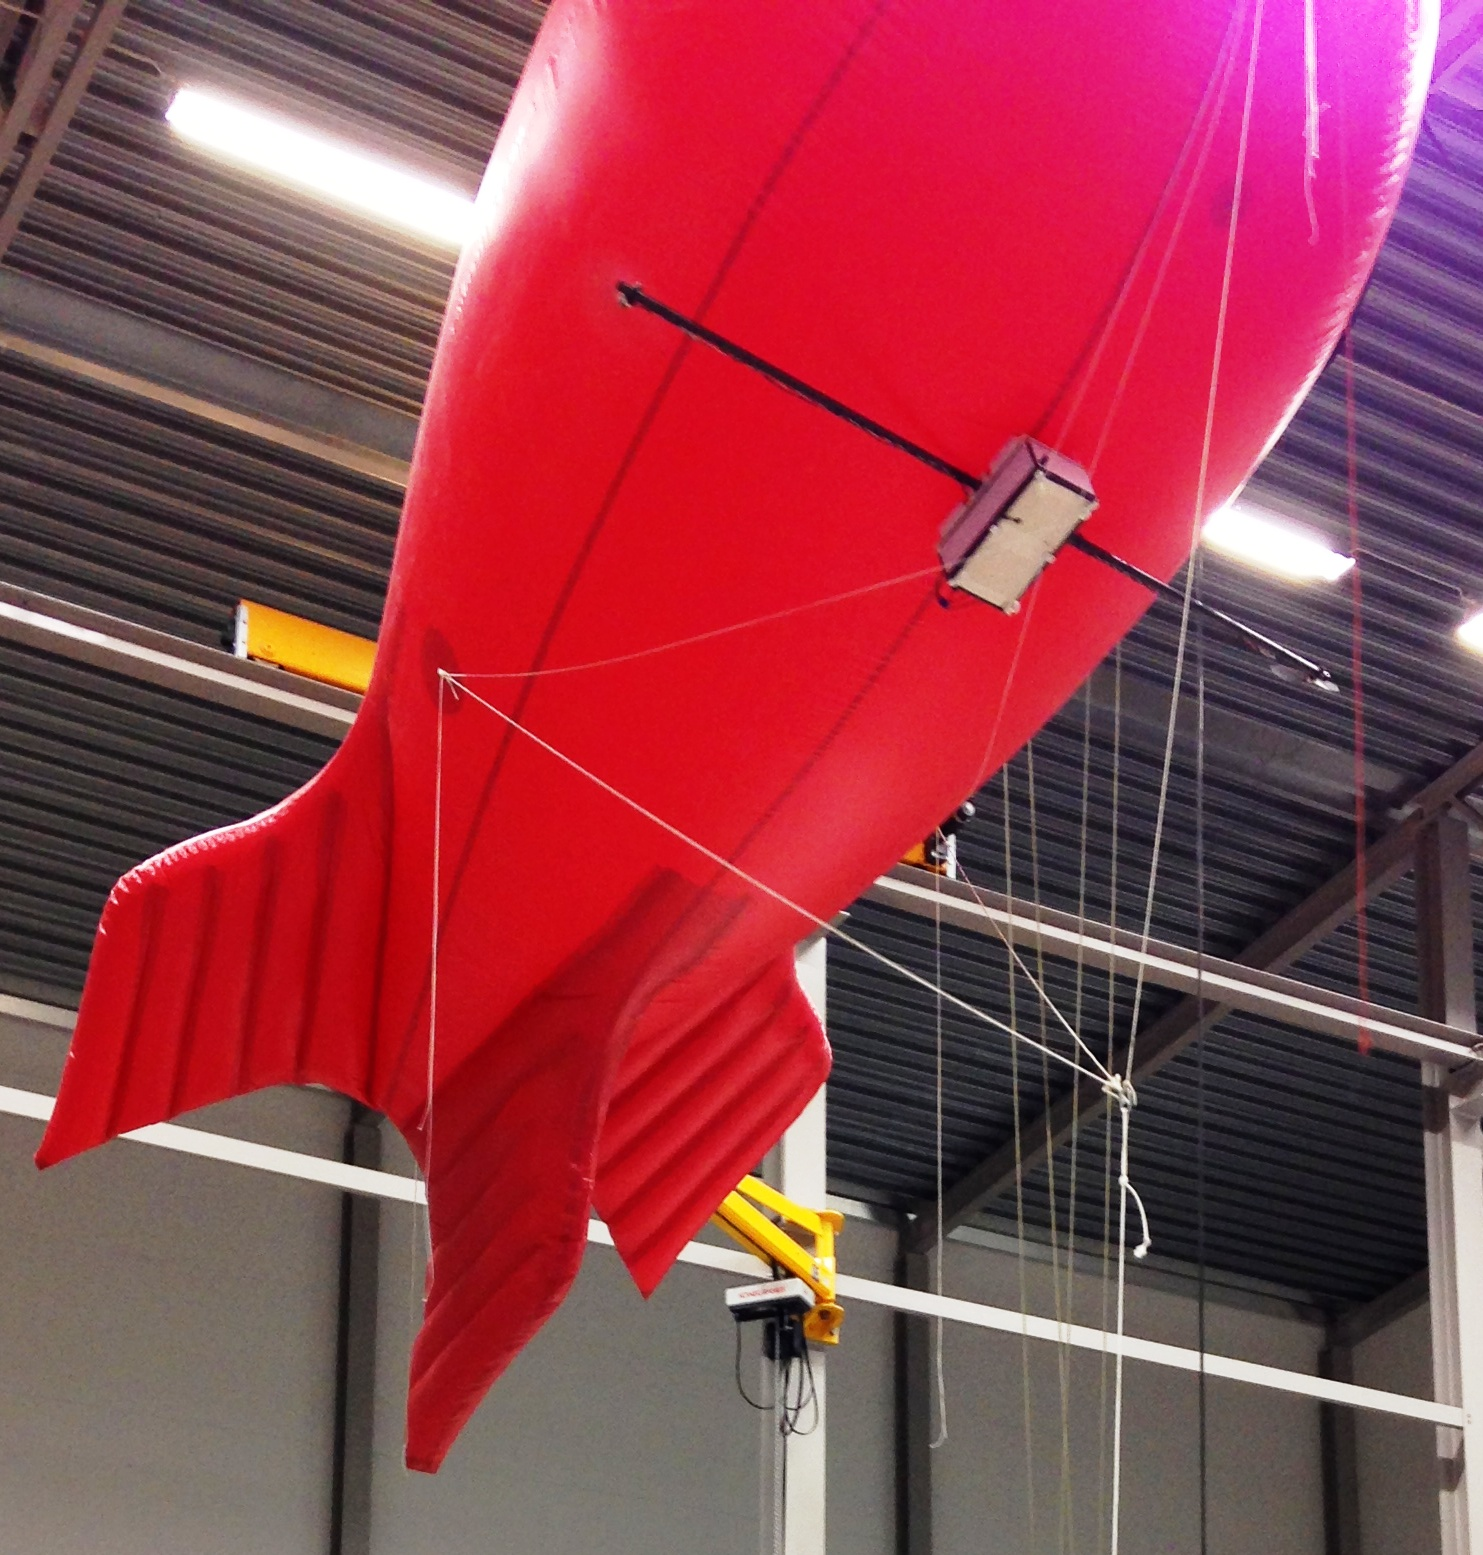
\includegraphics[width=0.7\textwidth]{figures/fig_FlightTest1_1}
\caption{First U-SPACE flight test}
\label{fig:FlightTest1_1}
\end{figure}
%
\begin{figure}[H]
\centering
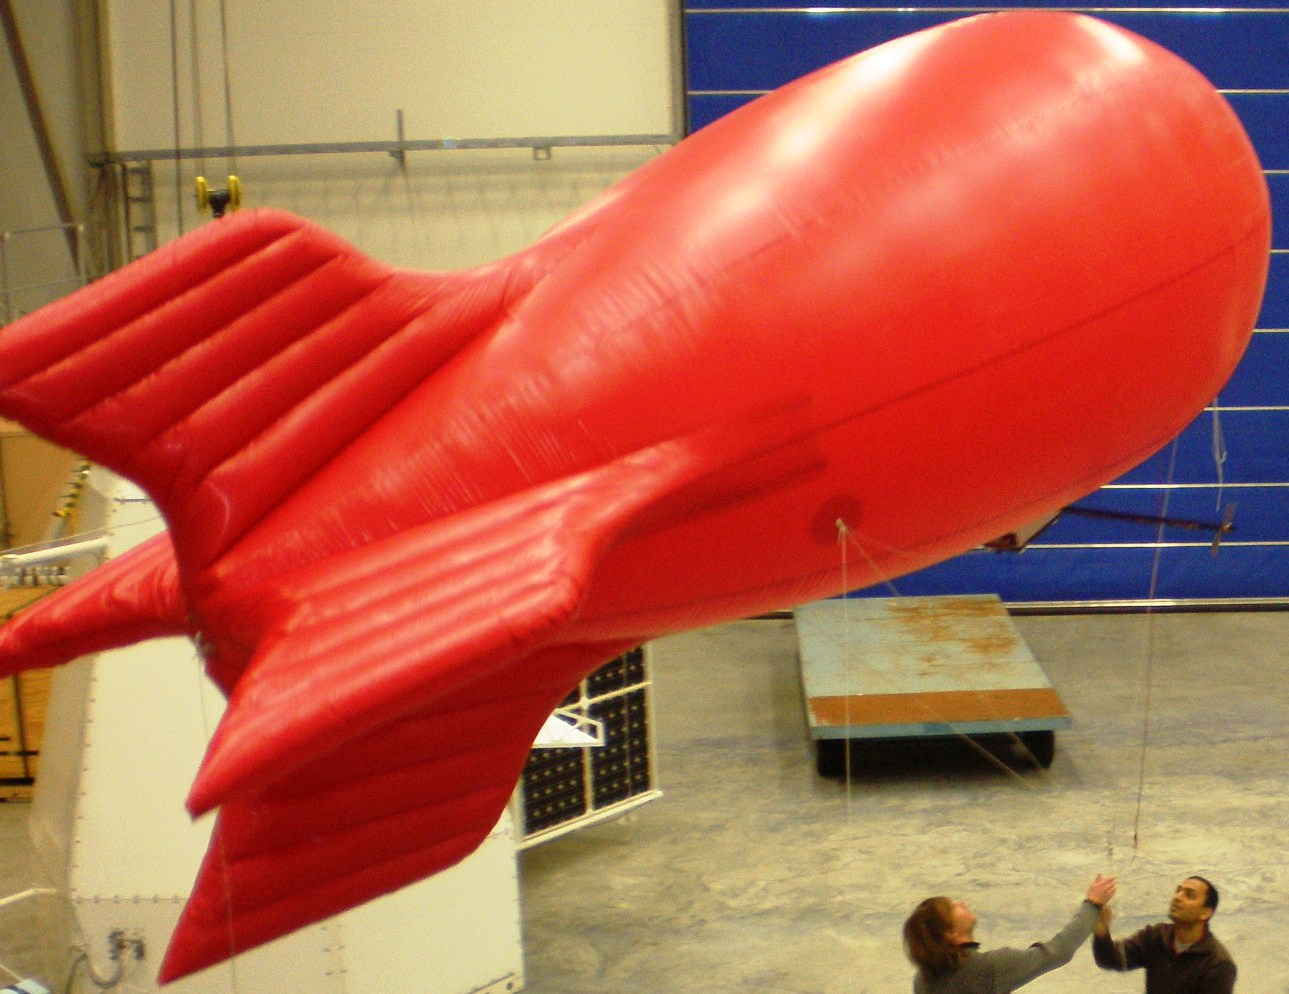
\includegraphics[width=0.7\textwidth]{figures/fig_FlightTest1_2}
\caption{First U-SPACE flight test}
\label{fig:FlightTest1_2}
\end{figure}
%
\subsection{Flight results for MCC}
At full throttle on the motors, we were able to propel the blimp forward and steer it to the side. However, it was clear that the amount of thrust generated by the motors was insufficient to properly propel the blimp. During the flight test, the blimp was attached to a concrete block on the ground via. a thin rope. When moving forward, the rope would stretch at an angle w.r.t. zenith and thus pull back the blimp. This made it difficult to estimate exactly the maximum velocity possible to obtain with the applied motor thrust. In this test, no attempt was made to "balance" out the lift of the blimp to the total mass of the U-SPACE systems. In future flights, it is recommended to balance out the lift using some dead weights (sand, small rocks etc.).


\subsection{Flight results for MSE}
%

\subsection{Flight results for ITPU}
%
Shortly before the flight test the BB failed. The attempted provisory fix using a BB-xM turned out to unstable during the flight test (see also \ref{sec:changes_itpu}). While trying to fixate cable connections between the BB-xM and the expansion board cable broke and damaged the expansion board unable to repair on the test side. Therefore the test results presented here are taken from the pre-flight test which was done in the facilities of LTU Kiruna when the original BB was still operational.

\begin{figure}
\centering
\includegraphics[width=0.55\textheight]{figures/full-system-setup}
\caption{Full system setup}
\label{fig:FlightTest1_1}
\end{figure}

An image of the full system setup including all electronical moduels can be seen in figure . This setup was then mounted into the payload box (see \textcolor{red}{REF!!!}) for testing. As mentioned in section \ref{sec:changes_itpu}, operating both the ADCs of the telemetry subsystem and the sensors of the attitude determination subsystem on the same I2C-bus caused problems which needed manual reset of the I2C-bus in order to get it working again. Peculiar was that both system worked when only one of the two ADCs where connected to the I2C bus together with the attitude sensors, but failed when both ADCs were connected. As the attempts to enable a second I2C-bus on a different expansion header of the BB were unsuccessful, it was decided to test only with one ADC and in turn loose 8 of the 16 telemetry values of the internal voltages. 

With this decision implemented the testing went successful. The wireless connection to the groundstation could be established (for more see \textcolor{red}{REF TO OMAIR}). After calibration of the magnetometer, the attitude determination system was able to determine the attitude stabily and produce the roll-, pitch- and yaw-angles for the telemetry system. When receiving the corresponding signal from the communication module the camera could be activated and shoot either single images or multiple images with a set period (fastest 1~s) and save them to the onboard sd-card.  


\section{Discussions and Future Recommendations}
%write for each subsystem
%
\subsection{EPS}
Due to the connector issues discussed in section \ref{sec:flight_results}, no telemetry was available during flight, thus detailed information of power consumption were not obtained. However, at full thrust, the system has in laboratory shown to draw around 2 x 7.5 A. At a voltage of approximately 7.0 V this corresponds to 105 W power delivered to the motors. In \cite{CDR} the \ac{EPS} was designed to deliver minimum 40 W of continuous solar power. With these flight results, to allow continuous flight, future designs should increase the solar array power output by at least a factor 2.5-3.
 
The \ac{BCR} should be re-designed for higher voltage and current outputs. Options for this were discussed in section \ref{sec:changes_BCR}. This also requires a battery pack with higher voltage. An advantage with higher voltage is that the power distribution efficiency is increased, since the diode voltage-drop losses and resistive losses ($I^2 \times R$) are relatively reduced when comparing to the total amount of handled power. 
%
\subsection{MCC}
From the previous discussed flight results, it was shown that the amount of generated thrust was just barely able to move the blimp. According to \cite{website:ModelMotors}, the motors have a relatively poor efficiency of around 67\%, especially when operating at heavy loads (high currents + low \ac{RMP}). The TIF-250 blimp from Esrange has a volume of $15 m^3$ and thus an approximate lift of around 15 kg. Including the motor efficiency, the power-to-lift ratio is 4.7 W/kg. Calculating this ratio for the Zeppelins that flew during the 1930's\cite{website:graf_zeppelin} gives 15.4 W/kg for the LZ-129 Hindenburg and 19.2 W/kg for the LZ-127 Graf. Thus the U-SPACE design has a power-to-lift ratio about 3-4 times less than old commercial designs. This agrees well with the lack of motor power to properly propel the blimp. The Zeppelins were designed for a cruise speed around 125 km/h (35 m/s) which is of course faster than the U-SPACE requirement. For future designs, it is recommended to include more powerful motors designed for low speed, low \ac{RPM} and high torque like \cite{website:ModelMotors_AXI5360}. Larger motors will also require a larger solar array to provide the power.